\title{Bayesian Inference}

(This is just a recall of my notes on bayesian inference, because I always
forget Bayes rule.)

\section{Philosophical comment}

Consider the following sentence

\begin{quote}
\emph{The probability that tossing the coin~$X$ you get heads is~$51\%$}
\end{quote}

What does it mean, exactly?

This is an important and difficult question.  There is no scientific
consensus about the meaning of this sentence.  There are two, very different,
answers: the so-called~\emph{frequentist} and~\emph{bayesian} interpretations
of probability.

The {\bf frequentist} interpretation is that this sentence gives a precise
information about the coin~$X$.  It says that the coin is somewhat biased
towards heads and against tails, and that if you repeat this experiment a
huge amount of times, it is very likely that you'll get more heads than
tails.  Precisely, the ratio of heads to tails will~\emph{converge}
towards~$51/49$ as the number of tosses tends to infinity.

The {\bf bayesian} interpretation is that this sentence gives a precise
information~\emph{about you}, not about the coin~$X$.  It says that your
current state of knowledge leads you to believe that it is more likely that
on the next toss, you will get heads rather than tails.  More precisely, that
if you were to place a bet on that coin toss, you would bet~$51$ against~$49$
that the result is heads.

The frequentist interpretation is a statement about the physical world, thus
it can be either true or false.  If it is true, then the sentence that the
probability of heads is~$52\%$ must be false because they are incompatible.
Also the sentence that the probability of heads is~$51.00000000001\%$, must
be false.  However, notice that it would be very, very difficult to check
which one of these sentences is true and which one is false, just by doing
experiments.  Consider that instead of tossing a coin you toss an omelette,
and that it gets destroyed after the first toss.  Can this sentence still
have a meaning?  Will you be able to ever check whether it is true or false?
I find the frequentist interpretation very difficult to understand.  Please,
somebody explain it to me more clearly.  I cannot honestly write about it
without my text looking like a straw man argument.

The bayesian interpretation is a statement about your personal beliefs, so it
does not really make sense to say that it is true or false.  Notice, in
particular, that the bayesian interpretation does not talk about the physical
world itself, only about your knowledge of this world.  The physical world
itself is deterministic.  The coin will land head or tails according to its
initial position and speed, following the deterministic laws of nature.  It
is only because you do not know with enough precision the position, speed,
and all the necessary physical details that you cannot be sure whether it
will land head or tails.
%But that is your problem.

What can you do, then, with a sentence about your personal beliefs?  Can you
do science with it?  Yes, you can.  The only thing that you can do is run
experiments and update your beliefs, after looking at the results of the
experiments.  This is what bayesian inference is all about: you have some
prior beliefs and you update them using the basic laws of probability theory.

\section{Bayes Formula}

The definition of conditional probability is
$$
P(A|B)=\frac{P(A\cap B)}{P(B)}
$$
then, by simple algebraic manipulation, and using different letters, you
obtain Bayes formula:
$$
P(\theta|D)=\frac{P(D|\theta)P(\theta)}{P(D)}
$$

You can interpret this formula in the following way

\begin{itemize}
	\item[$D$] the observed data
	\item[$\theta$] the parameters
	\item[$P(\theta)$] your \emph{prior} knowledge about the parameters
	\item[$P(\theta|D)$] your knowledge about the parameters after having
		observed the data (the \emph{posterior})
	\item[$P(D|\theta)$] the ``generative model'': given a value of the
		parameters, what is the distribution distribution of the data?
	\item[$P(D)$] a normalization factor equal to~$\int
		P(D|\theta)P(\theta)\mathrm{d}\theta$.
\end{itemize}

This formula tells you how to update your prior knowledge~$P(\theta)$ about
the parameters~$\theta$ after having observed the data~$D$.  For that, you
need to take into account the ``data generation model'', that describes how
likely is each datum for a given value of the parameters.

\section{Examples of inference}

The only way to understand inference is doing some simple examples.

\subsection{Inference for quiche-eaters}

Let us start with the easiest possible inference problem.

Let us suppose that an experiment produces independent samples of a normally
distributed random variable of mean~$\mu$ and standard deviation~$\sigma$.
We have observed~$N$ samples of values~$x_1,\ldots,x_N$.  What can we say
about~$\mu$ and~$\sigma$?

If you have had some exposure to~\emph{estimation theory}, you would
automatically say, we define~\emph{estimators} for the unknown parameters,
such as
$$
\hat\mu :=\frac{1}{N}\sum_{n=1}^N x_n
$$

and

$$
\hat\sigma_1 :=\sqrt{\frac{1}{N}\sum_{n=1}^N (x_n-\hat\mu)^2}
$$

or maybe

$$
\hat\sigma_2 :=\sqrt{\frac{1}{N-1}\sum_{n=1}^N (x_n-\hat\mu)^2}
$$

or even, god forbid,

$$
\hat\sigma_3 :=\sqrt{\frac{1}{N-1.5}\ \sum_{n=1}^N (x_n-\hat\mu)^2}
$$

or, if you are really fancy, you can use an~\emph{unbiased} estimator
for~$\sigma$

$$
\hat\sigma_4
:=\frac{\Gamma\left(\frac{n-1}{2}\right)}{\Gamma\left(\frac{n}{2}\right)\sqrt{2}}\ \sqrt{\sum_{n=1}^N (x_n-\hat\mu)^2}
$$

There are more unbiased estimators for~$\sigma$, this one is just an example.
Where do these fantastic formulas come from? From heuristics, mostly.  You
invent them, and then you prove some properties about them: such as being
unbiased, or having minimal variance, and whatnot.  This is some serious
bullshit that you should avoid as much as possible.  This strong language is
not used lightly.  The notion of ``unbiased estimator'' is
nonsensical because it does not commute with changes of units.  An estimator
of fuel consumption can be biased in miles per gallon, but unbiased in liters
per kilometer, or vice-versa!  Often, you can pick a biased estimator, apply
an appropriate functional transformation to it and then it becomes unbiased.
For example, using the notation above, the estimators~$\hat\sigma_4$
and~$\hat\sigma_2^2$ are unbiased estimators for~$\sigma~$ and~$\sigma^2$
respectively; however,~$\hat\sigma_2$ and~$\hat\sigma_4^2$ are biased
estimators for~$\sigma$ and~$\sigma^2$.  Thus, the fact of being unbiased
depends on whether we use linear or quadratic units, not on the computation
itself!

\subsection{How real men do inference}

Let us start again with the easiest possible inference possible: to
estimate~$\mu$ and~$\sigma$ from independent observations~$x_1,\ldots,x_N$ of
a normal random variable.  What can we do?  We can state what we do know:

(1) We know that the values~$x_1,\ldots,x_N$ are independent samples of a
random variable of type~$\mathcal{N}(\mu,\sigma)$.

(2) We do not know anything about~$\mu$

(3) We do not know anything about~$\sigma$

Well, if that is really the case, I have bad news: there's nothing that we
can do!

\begin{quote}
	\emph{You can't do inference---or data compression---without
	making assumptions.}\newline
	--David~J.~C.~MacKay
\end{quote}

And that's it.  Bayesian inference does not allow you to infer
anything from raw data alone.  If you want to do inference, you have to begin with
some~\emph{prior knowledge} (that may be as imprecise as you want), and then,
after having observed the data, you use Bayes rule to~\emph{update} your
knowledge according to the observations.

Since your knowledge, or lack thereof, is always modelled by probability
distributions, you have to specify a prior probability
distribution for your unknown parameters~$\mu$ and~$\sigma$.  For example,
you can suppose, that~$|\mu|\le10^6$ and
that~$0\le\sigma\le10^6$.  More precisely, we assume that~$\mu$ and~$\sigma$
are independent and that they have uniform distributions in the indicated
intervals.  This is then the prior density distribution of the parameters, that
models our knowledge before observing any data:
$$
P(\mu,\sigma)=P(\mu)\cdot P(\sigma)=
\frac{1}{2\cdot10^6}\mathbf{1}_{\left[-10^6,10^6\right]}(\mu)
\cdot
\frac{1}{10^6}\mathbf{1}_{\left[0,10^6\right]}(\sigma)
$$
This is our model for the prior: a constant function on a huge rectangle of
the plane.

More interesting is the data generation model:
$$
P(x_1,\ldots,x_N|\mu,\sigma)=
\prod_{n=1}^N \frac{1}{\sigma\sqrt{2\pi}}e^{-\frac{(x_n-\mu)^2}{2\sigma^2}}
$$
this formula is the exact translation of the sentence ``the~$x_n$ are
independent, identically distributed samples of~$\mathcal{N}(\mu,\sigma)$''.
By simple manipulation, the formula above is written as
$$
P(x_1,\ldots,x_N|\mu,\sigma)=
\sigma^{-N}(2\pi)^{-N/2}\exp\left(-\sum_{n=1}^N\frac{(x_n-\mu)^2}{2\sigma^2}\right)
$$

Now, Bayes rule says
$$
P(\mu,\sigma|x_1,\ldots,x_N)=
P(x_1,\ldots,x_N|\mu,\sigma)\cdot P(\mu,\sigma)/Z
$$

Where~$Z$ is a constant such that the integral of~$P$ is~$1$.
For a given set of data points~$x_1,\ldots,x_N$, this is a function of two
variables~$(\mu,\sigma)$ that you can evaluate, plot and study.
You better get used to these plots, because they are the final output of the
inference.  There's nothing else to do!

\begin{tabular}{ll}
	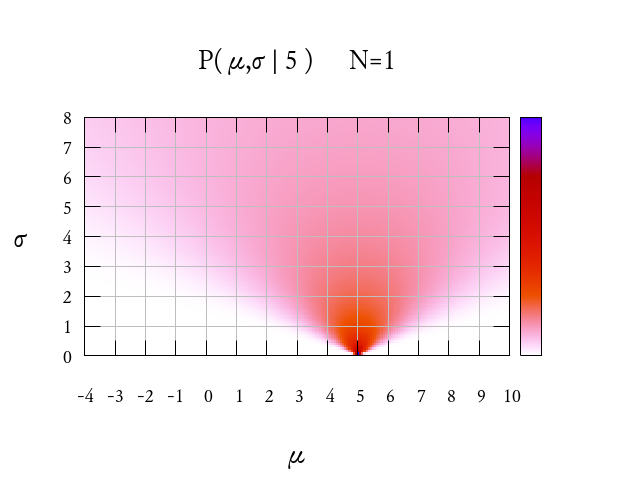
\includegraphics{bayes1.png}&
	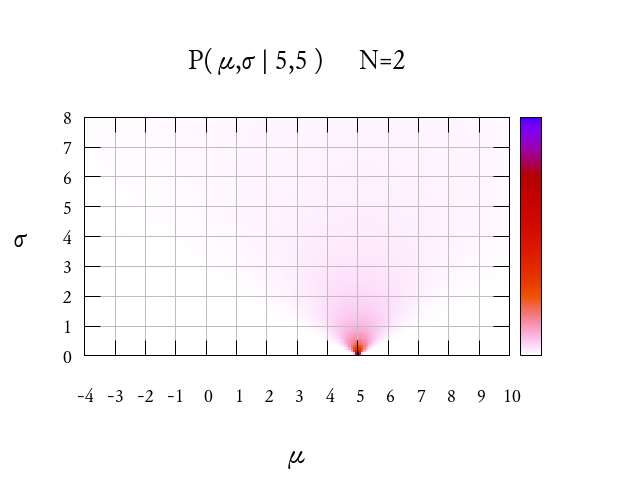
\includegraphics{bayes2.png}\\
	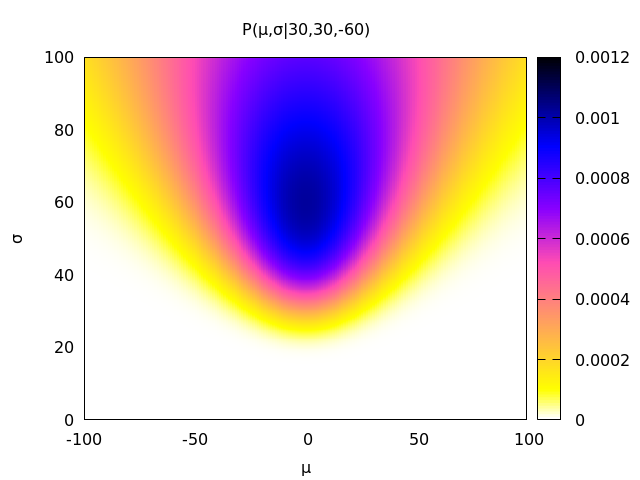
\includegraphics{bayes3.png}&
	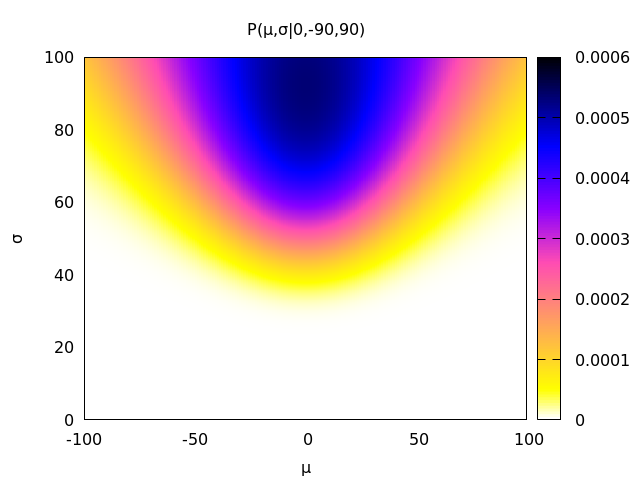
\includegraphics{bayes4.png}\\
	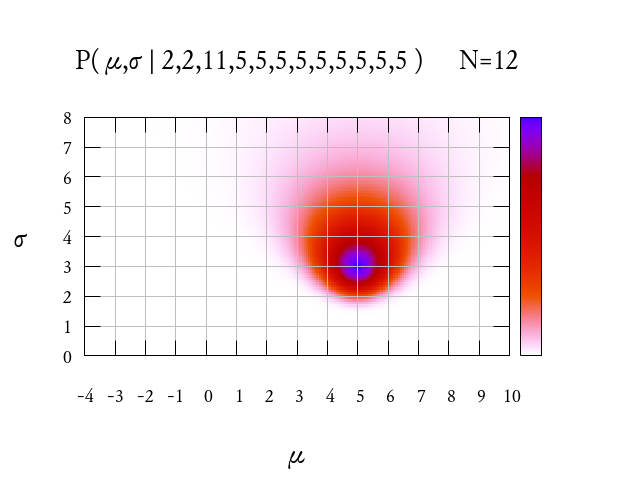
\includegraphics{bayes5.png}&
	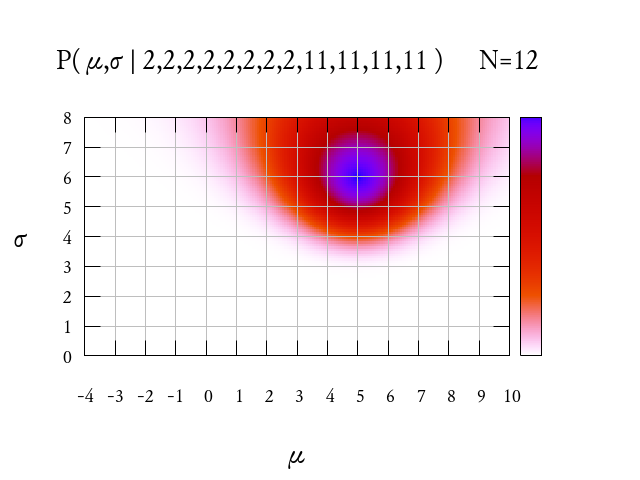
\includegraphics{bayes6.png}\\
\end{tabular}
%SCRIPT cat <<END >gmap.g
%SCRIPT set term pngcairo font "Junicode,20"
%SCRIPT set isosample 100,100
%SCRIPT set samples 200
%SCRIPT f(m,s)=s**(-|a|)*exp(-(sum [i=1:|a|] (a[i]-m)**2)/(2*s**2))
%SCRIPT set xrange [-4:10]
%SCRIPT set yrange [0:8]
%SCRIPT set xtics 1 font ",14"
%SCRIPT set ytics 1 font ",14"
%SCRIPT unset key
%SCRIPT set grid front xtics ytics lw 1 lt -1 lc rgb 'gray'
%SCRIPT set table 'caca.dat'
%SCRIPT splot f(x,y)
%SCRIPT unset table
%SCRIPT set title sprintf("P( μ,σ | %s )     N=%d",t,|a|)
%SCRIPT set xlabel "μ"
%SCRIPT set ylabel "σ" rotate by 0
%SCRIPT unset cbtics
%SCRIPT set palette rgbformulae 8,6,16 negative
%SCRIPT plot 'caca.dat' with image
%SCRIPT END

%SCRIPT X="5"           ;gnuplot -e "array a[1]=[$X];t='$X'" gmap.g >bayes1.png
%SCRIPT X="5,5"         ;gnuplot -e "array a[2]=[$X];t='$X'" gmap.g >bayes2.png
%SCRIPT X="4,4,7"       ;gnuplot -e "array a[3]=[$X];t='$X'" gmap.g >bayes3.png
%SCRIPT X="2,2,11"       ;gnuplot -e "array a[3]=[$X];t='$X'" gmap.g >bayes4.png
%SCRIPT X="2,2,11,5,5,5,5,5,5,5,5,5"
%SCRIPT gnuplot -e "array a[12]=[$X];t='$X'" gmap.g >bayes5.png
%SCRIPT X="2,2,2,2,2,2,2,2,11,11,11,11"
%SCRIPT gnuplot -e "array a[12]=[$X];t='$X'" gmap.g >bayes6.png

TODO: write some comments about the interpretation of each plot above.


In rare occasions, you may want to summarize the whole posterior
distribution~$P(\mu,\sigma|\ldots)$ by a single representative
point~$(\mu,\sigma)$.  There are several ways to do that.  For example, you
can pick the mean value of this distribution, or some sort of median, or the
position of the maximum.  You can also integrate along one variable, and take
the maximum of this integral with respect to the other.  This is actually
done and there are whole books about how to compute these integrals (this is
called~\emph{marginalization}).  These are all examples
of---gasp---\emph{estimators}; that is, functions of the
form~$(x_1,\ldots,x_N)\mapsto(\mu,\sigma)$.  Estimators are sometimes useful,
if you want a fast summary of the posterior distribution.  However, they
should never be used as an intermediate product in a chain of inferences.
You should always keep the whole distribution and update it as new data
arrives!

In many cases, the easiest estimator to compute is the position maximum
value, also called the~\emph{mode} or the maximum a-posteriori (``MAP'').
This is because we know that the function~$P(\mu,\sigma|\ldots)$ is smooth,
and the extrema of smooth functions can be found by differentiation.

For the example of the normal, we want to find the extrema of this
function:
$$
f(\mu,\sigma)
=
\sigma^{-N}\exp\left(-\sigma^{-2}\sum_{n=1}^N\tfrac{1}{2}(x_n-\mu)^2\right)
$$
which is trivial to optimize by using the conditions~$f_\mu=f_\sigma=0$.
The explicit computation follows:
$$
f_\mu(\mu,\sigma)
=
\sigma^{-N}\exp\left(-\sigma^{-2}\sum_{n=1}^N\tfrac{1}{2}(x_n-\mu)^2\right)
\left[
	-\sigma^{-2}\sum_{n=1}^N(x_n-\mu)
\right]
$$
then~$f_\mu=0$ is equivalent to
$$
0 = \sum_{n=1}^N(x_n-\mu)
$$
which in turn is equivalent to
$$
\mu=\frac{1}{N}\sum_{n=1}^Nx_n.
$$
Thus, the MAP estimator in this case coincides with the ``traditional''
estimator of the mean.  Everything is alright.

Now let us perform the corresponding computation for~$\sigma$:
$$
f_\sigma(\mu,\sigma)
=
-N\sigma^{-N-1}\exp\left(...\right)
+\sigma^{-N}\exp\left(...\right)
\left[
	2\sigma^{-3}\sum_{n=1}^N\tfrac{1}{2}(x_i-\mu)^2
\right]
$$
so that~$f_\sigma=0$ is equivalent to
$$
N\sigma^{-N-1}
=
\sigma^{-3-N}\sum_{n=1}^N(x_i-\mu)^2
$$
and solving for~$\sigma$:
$$
\sigma=\sqrt{\frac{1}{N}\sum_{n=1}^N(x_i-\mu)^2}
$$
which is the estimator usually called~$\bar\sigma_{N}$.  Looking at the
plots above we see why an estimator for~$\sigma$ ought to be larger
than~$\bar\sigma_{N}$: the distribution is heavily skewed in the vertical
direction: the $\sigma$-position of the maximum is lower than the average
value.

\bigskip

The result of our inference is a probability
distribution~$f(\mu,\sigma)=P(\mu,\sigma|x_1,\ldots,x_N)$.  The
function~$f(\mu,\sigma)$ can be interpreted and used in many ways.  The
following constructions extract a single value~$(\mu,\sigma)$ from
the posterior distribution:

\begin{enumerate}
	\item As a \emph{joint posterior  distribution}: the value
		of~$f(x,y)$ is a measure of our belief that~$\mu=x$
		and~$\sigma=y$ after having observed the data.
	\item The mode of~$f(\mu,\sigma)$:
		$$
		\arg\max_{(\mu,\sigma)}\ f(\mu,\sigma)
		$$
		is the value of~$(\mu,\sigma)$ that is more probable.
		It is called the~\emph{maximum a-posteriori} (MAP) estimator
		of~$(\mu,\sigma)$.
	\item The mean of~$f(\mu,\sigma)$:
		$$
		\int (\mu,\sigma)f(\mu,\sigma)
		\,\mathrm{d}\mu
		\,\mathrm{d}\sigma
		$$
		is called the~\emph{minimum mean square error} (MMSE).
		It has this name because it minimizes a quadratic error
		called the ``squared error risk''.
	\item More generally, you can take a parameter~$p>0$ and define
		the~$p$-risk which is the~$p$-norm of the error.  The MMSE
		and the MAP arise as particular cases for~$p=2$ and~$p\to0$,
		and it yields the~\emph{posterior median estimator}
		for~$p=1$.
\end{enumerate}

And the following constructions extract a function of one variable from the
posterior distribution:

\begin{enumerate}
	\item Fixing a value of~$\mu$, the function
		$$
		g(\sigma)=\frac{f(\mu,\sigma)}{\int_0^\infty
		f(\mu,y)\,\mathrm{d}y}
		$$
		is the \emph{conditional probability} of~$\sigma$ given~$\mu$
		and the data.  Formally, the function~$g$ is obtained by
		evaluating~$f$ along vertical lines, with a normalization
		factor so that the integral is 1.
		This conditional probability answers the question ``what do
		we know about~$\sigma$ given that we know~$\mu$?''
	\item We can also average over all possible values of~$\mu$, to
		obtain the function
		$$
		h(\sigma)=\int_{-\infty}^\infty
		f(\sigma,\mu)\,\mathrm{d}\mu
		$$
		this function has integral 1 so it is a probability
		distribution, called the~\emph{marginal distribution}
		of~$\sigma$.  Formally, the function~$h$ is obtained by
		projecting the whole plot into a vertical line.
		The marginal probability answers a very different question
		than the conditional: ``what do we know about~$\sigma$, if we
		know nothing about~$\mu$?''
	\item Similarly, we can exchange the roles of~$\mu$ and~$\sigma$ on
		the previous two functions to obtain the posterior~$\mu$
		conditional to a value of~$\sigma$
		$$
		\mu\mapsto\frac{f(\mu,\sigma)}{\int_{-\infty}^\infty
		f(x,\sigma)\,\mathrm{d}x}
		$$
		and the marginal distribution of~$\mu$
		$$
		\mu\mapsto\int_0^\infty
		f(\mu,\sigma)\,\mathrm{d}\sigma
		$$
\end{enumerate}

Finally, we can compute estimators (MAP,MMSE,$\ldots$) of each of these
one-dimensional distributions.
For the case of the normal model, all these possibilities are well known
and tabulated, because the integrals can be computed in closed form.  But you
can nearly always compute them numerically: modern CPUs are very fast.

The functional notation~$f(\mu,\sigma)$,~$g(\sigma)$ etc. are practical for
computations on paper but they are rarely used in print, where the following
notation is preferred (where~$Z$ denotes whatever normalization factor is
needed so that the integral is 1).

The posterior probability of~$\mu$ given~$\sigma$:
$$
P(\mu|x_1,\ldots,x_N,\sigma)=P(x_1,\ldots,x_N|\mu,\sigma)P(\mu)/Z
$$
in the case of a normal with non-informative priors this turns out to be a
normal
distribution~$P(\mu|\cdots)\sim\mathcal{N}\left(\bar{x},\sigma^2/N\right)$.

The marginal probability of~$\mu$ is
$$
P(\mu|x_1,\ldots,x_N)=P(x_1,\ldots,x_N|\mu)P(\mu)/Z
$$
which, in the case of a normal with non-informative priors is a Student-$t$
distribution~$P(\mu|\cdots)\sim\left(N(\mu-\bar
x)^2+\sigma_{{}_N}^2\right)^{-N/2}$.
This is a very important and useful formula.  It answers the question~``given
the samples, what do we know about~$\mu$?''.

Consider now the typical notations in scientific calcutators:
$$
\bar x=\frac{\sum_{n=1}^nx_n}{N}
\qquad
\sigma_{{}_N}=\sqrt{\frac{1}{N}\sum_{n=1}^n(x_n-\bar x)^2}
\qquad
\sigma_{{}_{N-1}}=\sqrt{\frac{1}{N-1}\sum_{n=1}^n(x_n-\bar x)^2}
$$

We have computed above that~$(\bar
x,\sigma_{{}_N})=MAP(P(\mu,\sigma|x_1,\ldots,x_n))$.
How can we get to~$\sigma_{{}_{N-1}}$?  Well, it turns out that
$
\sigma_{{}_{N-1}}=MAP(P(\sigma|x_1,\ldots,x_N)).
$
(the estimator~$\sigma_{{}_{N-1}}$ is the mode of the posterior marginal
distribution of~$\sigma$).  Thus, $\sigma_{{}_{N-1}}$ appears naturally in a
probabilistic setting, as one of the natural quantites that we can extract
from our inference.
%Notice, however, that the MAP is not invariant by changes of variable in the
%domain, so that the same scathing criticism that we did to the definition of
%``unbiased'' estimator can be applied here as well.
% ENRIC: clarify, it actually IS invariant! (but you have to measure the
% density with respect to the radom/nikodym derivative of the measures)
% thus, by fixing a riemannian structure on the domain, and computing
% derivatives of measures wrt to it, the MAP and MMSE are indeed invariant.
% ENRIC2: in any case, the ML estimator *is* always invariant, so using
% non-informative priors the estimators are actually invariant.

Let us give the details of this computation.  We have, up to a constant, the
following joint distribution
$$
f(\mu,\sigma)=\sigma^{-N}\exp\left(
-\sigma^{-2}\sum_{n=1}^N\tfrac{1}{2}\left(x_n-\mu\right)^2
\right)
$$
and we want to locate the maximum of the marginal distribution
$$
g(\sigma)=\int_{-\infty}^\infty f(\mu,\sigma)\,\mathrm{d}\mu
$$
For that, we rewrite the function~$f$ in a more convenient form where the
parameter~$\mu$ appears only once.  We use the
well-known expression~$\sigma_{{}_N}^2=\frac{\sum x_n^2}{N}-\bar x^2$,
and~$f$ is then simplified to
$$
f(\mu,\sigma)=\sigma^{-N}\exp\left(
-\sigma^{-2}\tfrac{N}{2}\left[(\mu-\bar x)^2+\sigma_{{}_N}^2\right]
\right)
$$
and so
$$
f(\mu,\sigma)=\sigma^{-N}\exp\left(
-\tfrac{\left(\mu-\bar x^2\right)}{2\left(\sigma/\sqrt{N}\right)^2}
\right)
\exp\left(-\sigma^2\tfrac{N}{2}\sigma_{{}_N}^2
\right)
$$
we have to integrate this last expression with respect to~$\mu$ to obtain the
function~$g(\sigma)$; only the middle factor depends on~$\mu$, and this
factor is a gaussian function of~$\mu$ of size~$\sigma/\sqrt{N}$, thus its
integral equals~$\sqrt{2\pi N}/\sigma$, so that
$$
g(\sigma)
=
\int_{-\infty}^\infty f(\mu,\sigma)\,\mathrm{d}\mu
\ \propto\ %
\sigma^{-N}\sqrt{N}e^{-\sigma^2\frac{N\sigma_N^2}{2}}
$$
the maximum will be found at a point~$\sigma$ such that~$g'(\sigma)$
and this condition simplifies to~$\sigma=\sigma_{N-1}$.



% vim:set tw=77 filetype=tex spell spelllang=en:
